%%%%%%%%%%%%%%%%%%%%%%%%%% Packages / Definitions %%%%%%%%%%%%%%%%%%%%%%%%%%%%
%
\documentclass{webofc}
\PassOptionsToPackage{}{xcolor}
\usepackage{xcolor}
\usepackage[varg]{txfonts}
\RequirePackage{orcidlink}
\usepackage{tikz}
\usetikzlibrary{calc, positioning, arrows.meta, fit}
\definecolor{listingbg}{RGB}{245,245,245}
\definecolor{user}{RGB}{79,129,189}
\usepackage[newfloat]{minted}

\setminted{
    bgcolor=listingbg,
    fontsize=\footnotesize,
    fontfamily=tt,
    breaklines=true,
    breakanywhere=false,
    frame=single,
    framesep=6pt,
    rulecolor=\color{user},
    linenos=true,
    firstnumber=1,
    numbersep=5pt,
    stepnumber=2,
    tabsize=2,
    obeytabs=true,
    showspaces=false,
    showtabs=false,
    autogobble=true,
    escapeinside=\%*\*),
}

\definecolor{problemred}{RGB}{140, 62, 84}   % muted red, print-safe

\tikzset{
  problemnote/.style={note, text=problemred},
  problemarrow/.style={drift, draw=problemred}
}

%%%%%%%%%%%%%%%%%%%%%%%%%% Document %%%%%%%%%%%%%%%%%%%%%%%%%%%%

\begin{document}
\title{An IaC-Framework for the future of CERN's Infrastructure and Configuration Management}

\author{\firstname{Christopher} \lastname{Barnes}\orcidlink{0009-0003-1963-7992}\inst{1}\fnsep\thanks{\email{christopher.barnes@cern.ch}} \and
        \firstname{Daniel} \lastname{Juárez}\orcidlink{0000-0000-0000-0000}\inst{1}\fnsep\thanks{\email{daniel.juarez@cern.ch}} \and
        \firstname{Luis} \lastname{Fernandez Alvarez}\orcidlink{0000-0000-0000-0000}\inst{1}\fnsep\thanks{\email{luis.fernandez.alvarez@cern.ch}} \and
        \firstname{Giacomo} \lastname{Tenagali}\orcidlink{0000-0000-0000-0000}\inst{1}\fnsep\thanks{\email{giacomo.tenagali@cern.ch}}
}

\institute{CERN, Esplanade des Particules 1, 1217 Meyrin, Switzerland}

\abstract{At CERN, provisioning, configuration, and operational state are each handled by a different system. Since 2012 the IT department has worked to bridge them under the Agile Infrastructure project, combining OpenStack, Puppet, and Foreman with a set of in-house services so that users see one coherent platform.

The result is mature, but the seams between these systems are still where the work goes. Traceability and reproducibility suffer most when a service is deployed for the first time, scaled up, or rebuilt after a failure. Exposing newer cloud features, such as load balancers or security groups, means writing another integration each time.

Infrastructure-as-Code (IaC) tools such as Terraform and its open-source fork, OpenTofu, offer a declarative and version-controlled model that can sit across these procedures. They also bring an ecosystem of off-the-shelf modules that can be reused rather than rebuilt.

We present a framework that plugs into the existing infrastructure and configuration management landscape through declarative definitions, custom providers for in-house services, and CI/CD pipelines that validate every change before it is applied. Using a set of case studies, we show where the framework cuts operational complexity, how it helps in disaster recovery, and what it adds in automation, auditability, and replication across environments, offering a foundation for the evolution of infrastructure and configuration management at CERN.
}

\maketitle

\section{Introduction}
\label{intro}

CERN runs a large computing infrastructure. Since 2012 the IT department has built up a configuration management (CM) system around Puppet and OpenStack, together with a number of in-house services, to manage its computing services~\cite{bellinfra2012}. Each of these tools does its own job well. What is missing is anything that ties them together, and the cost shows up in traceability, reproducibility, and maintainability.

Procedures for managing servers do exist. Keeping the service documentation in step with the infrastructure is the harder problem, particularly in an environment with frequent personnel rotation. When the person who set a service up is no longer around, recovering or reconfiguring it is slow. Because IaC tools are declarative, the desired state of the infrastructure is the documentation, which removes much of that dependency on institutional memory. There is a second gap as well: Puppet and tools like it manage the configuration of a server, not the server itself~\cite{loope2011managing}. When the machine underneath is degraded or gone, CM has nothing to converge.

Over the past few years IaC has become the standard model for consolidating how infrastructure is developed, deployed, and automated~\cite{morris2025infrastructure}. Terraform and its community-driven fork, OpenTofu, are the most widely used implementations, and both are a plausible basis for unifying provisioning and configuration in a reproducible and scalable way~\cite{holkuziev2025infrastructure}.

This work sets out to design and implement an IaC-based framework that integrates with the existing infrastructure management ecosystem rather than replacing it, and that gives operators a single automated and traceable way to manage resources spread across cloud regions. If the integration works, the payoff is less operational complexity and maintenance effort, better automation and reproducibility, and a far easier path through Business Continuity / Disaster Recovery (BC/DR) and cross-environment replication. We see it as a first step towards a more unified infrastructure management strategy at CERN.

\section{Current Infrastructure Landscape and Challenges}\label{infra}

CERN runs its own cloud on OpenStack~\cite{dupuis2025,savchenko2024preparing}. Around it sit several in-house services that manage machine state, trust, and network configuration~\cite{martelli2018}. Foreman acts as the central External Node Classification (ENC) system for Puppet, holding the hostgroup assignments, environments, and metadata that are consumed when a catalog is compiled.

Production systems are usually provisioned through an internal tool that wraps those services and creates the resources. A cloud-init script then bootstraps Puppet, which takes over lifecycle management of the machine. Once the Puppet agent makes its first catalog request, the host is in ongoing CM.

Terraform has already been used at CERN in a narrower scope. The Batch Service adopted it to bootstrap Kubernetes clusters, holding manifests in GitLab and applying them from CI/CD, having run into the same home-grown tooling that stitches OpenStack, Foreman, and Puppet together~\cite{alvarez2020batch}. That work established the pattern for a single service; what is missing is a model that covers provisioning across the estate.

The pain points here are not in the individual tools. They are in the interfaces between them. State lives in Foreman, in OpenStack, in alert management, in state management, and in a network database, and parts of it are duplicated or derived independently in more than one place. A change that propagates through several of these systems can leave them disagreeing, and someone has to go and fix it by hand. Figure~\ref{fig:state-boundaries} shows where those drift boundaries fall.

\begin{figure}[tbp]
  \centering
    \scalebox{0.88}{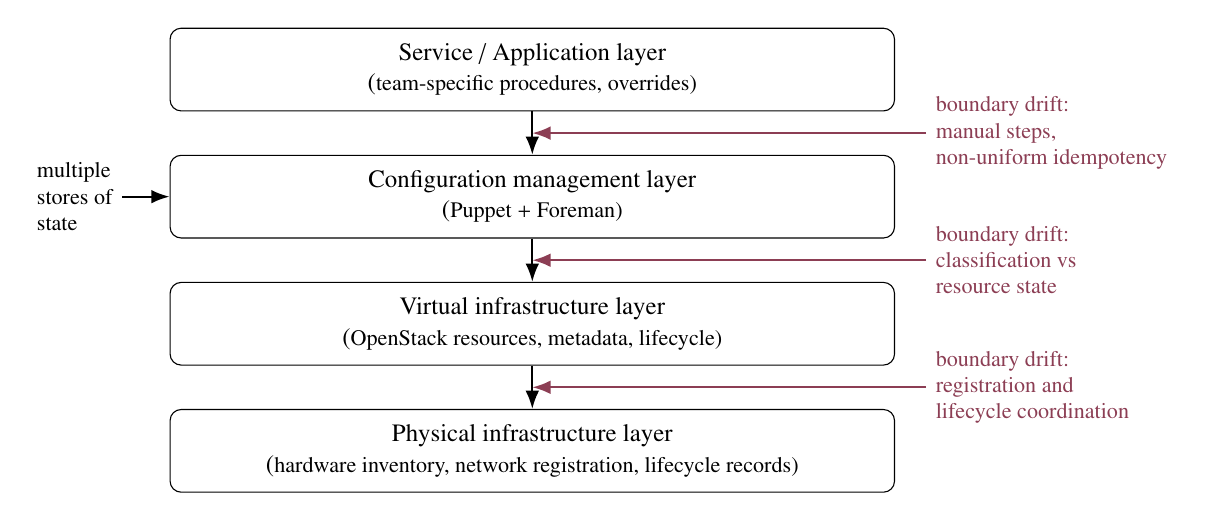
\begin{tikzpicture}[
    font=\small,
    box/.style={
        draw, rounded corners, align=center,
        minimum width=9.2cm, minimum height=1.05cm, inner sep=3pt
      },
    drift/.style={-Latex, thick},
    note/.style={align=left, font=\footnotesize},
    node distance=0.55cm
  ]

  \node[box] (svc) {Service / Application layer\\(\footnotesize team-specific procedures, overrides)};
  \node[box, below=of svc] (cm) {Configuration management layer\\(\footnotesize Puppet + Foreman)};
  \node[box, below=of cm] (cloud) {Virtual infrastructure layer\\(\footnotesize OpenStack resources, metadata, lifecycle)};
  \node[box, below=of cloud] (phys) {Physical infrastructure layer\\(\footnotesize hardware inventory, network registration, lifecycle records)};

  \coordinate (b1) at ($(svc.south)!0.5!(cm.north)$);
  \coordinate (b2) at ($(cm.south)!0.5!(cloud.north)$);
  \coordinate (b3) at ($(cloud.south)!0.5!(phys.north)$);

  \draw[drift] (svc.south) -- (cm.north);
  \draw[drift] (cm.south) -- (cloud.north);
  \draw[drift] (cloud.south) -- (phys.north);

  \node[problemnote, right=5cm of b1] (d1)
  {boundary drift:\\manual steps,\\non-uniform idempotency};
  \draw[problemarrow] (d1.west) -- (b1);

  \node[problemnote, right=5cm of b2] (d2)
  {boundary drift:\\classification vs\\resource state};
  \draw[problemarrow] (d2.west) -- (b2);

  \node[problemnote, right=5cm of b3] (d3)
  {boundary drift:\\registration and\\lifecycle coordination};
  \draw[problemarrow] (d3.west) -- (b3);

  \node[note, left=0.6cm of cm.west] (sot)
  {multiple\\stores of\\state};
  \draw[drift] (sot.east) -- (cm.west);

\end{tikzpicture}
}
  \caption{Layered view of the current infrastructure stack.}
  \label{fig:state-boundaries}
\end{figure}

Four limitations stand out. State representations overlap across systems and converge late. Change propagates asynchronously with weak end-to-end guarantees. Manual steps remain in provisioning, for registration, hardware tracking, and the exceptional workflows. And end-to-end observability is limited, so feedback loops are slow. The internal tool that most people use to deploy infrastructure is itself fire-and-forget: it runs no pre-flight checks on permissions or quota, and it fails silently.

What is absent is a single declarative model covering all of the artifacts involved, the virtual resources, the service-level configuration, and the supporting registrations. Without it, end-to-end automation stops short and convergence depends on coordinating across systems by hand. That is the gap a Terraform/OpenTofu-based framework is meant to close, by reducing boundary drift, making the layers idempotent, and making change traceable.

\section{Framework Design}\label{design}

\subsection{Architecture and Lifecycle Layers}
The framework is built around three lifecycle layers, each with its own scope. Figure~\ref{fig:framework-layers} shows where they meet the existing services.

\begin{figure}[tbp]
  \centering
    \scalebox{0.95}{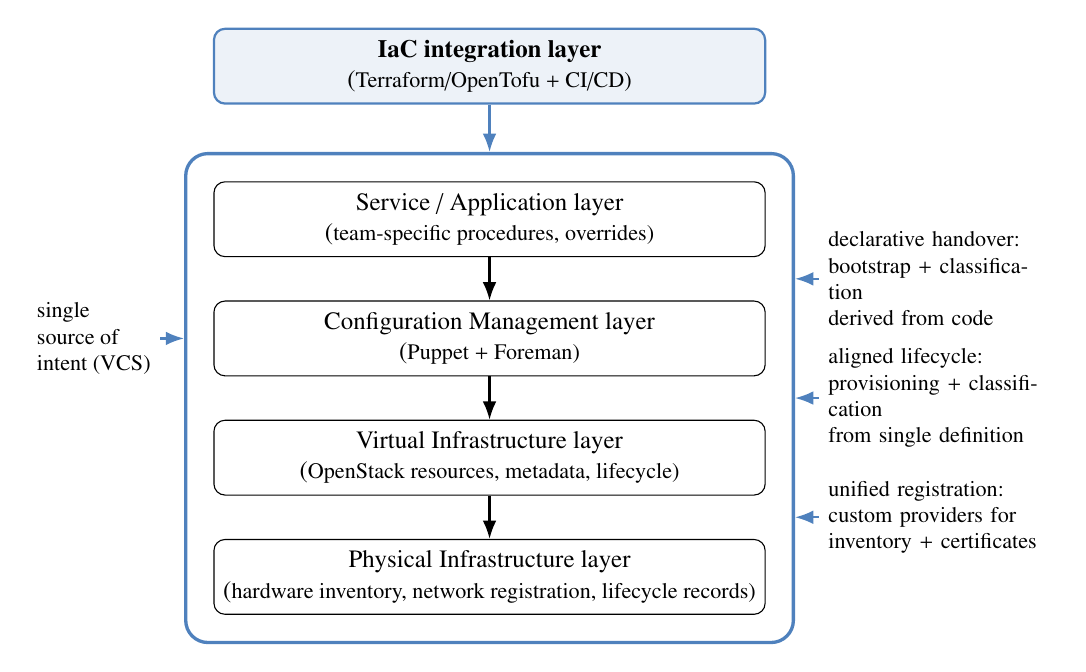
\begin{tikzpicture}[
    font=\small,
    box/.style={
        draw, rounded corners, align=center,
        minimum width=7.0cm, minimum height=0.95cm, inner sep=3pt
      },
    iacbox/.style={
        draw=user, thick, rounded corners, align=center,
        minimum width=7.0cm, minimum height=0.95cm, inner sep=3pt,
        fill=user!10
      },
    drift/.style={-Latex, thick},
    note/.style={align=left, font=\footnotesize},
    framebox/.style={
        draw=user, very thick, rounded corners=8pt,
        inner xsep=10pt, inner ysep=10pt
      },
    resolvenote/.style={align=left, font=\footnotesize, text width=2.8cm},
    resolvearrow/.style={-Latex, thick, draw=user},
    node distance=0.55cm
  ]

  \node[box] (svc) {Service / Application layer\\(\footnotesize team-specific procedures, overrides)};
  \node[box, below=of svc] (cm) {Configuration Management layer\\(\footnotesize Puppet + Foreman)};
  \node[box, below=of cm] (cloud) {Virtual Infrastructure layer\\(\footnotesize OpenStack resources, metadata, lifecycle)};
  \node[box, below=of cloud] (phys) {Physical Infrastructure layer\\(\footnotesize hardware inventory, network registration, lifecycle records)};

  \node[framebox, fit=(svc)(cm)(cloud)(phys)] (framework) {};

  \node[iacbox, above=0.6cm of framework.north] (iac) {\textbf{IaC integration layer}\\(\footnotesize Terraform/OpenTofu + CI/CD)};

  \draw[drift, draw=user] (iac.south) -- (framework.north);

  \coordinate (b1) at ($(svc.south)!0.5!(cm.north)$);
  \coordinate (b2) at ($(cm.south)!0.5!(cloud.north)$);
  \coordinate (b3) at ($(cloud.south)!0.5!(phys.north)$);

  \draw[drift] (svc.south) -- (cm.north);
  \draw[drift] (cm.south) -- (cloud.north);
  \draw[drift] (cloud.south) -- (phys.north);

  \node[resolvenote, right=0.3cm of framework.east |- b1] (d1)
  {declarative handover:\\bootstrap + classification\\derived from code};
  \draw[resolvearrow] (d1.west) -- (framework.east |- b1);

  \node[resolvenote, right=0.3cm of framework.east |- b2] (d2)
  {aligned lifecycle:\\provisioning + classification\\from single definition};
  \draw[resolvearrow] (d2.west) -- (framework.east |- b2);

  \node[resolvenote, right=0.3cm of framework.east |- b3] (d3)
  {unified registration:\\custom providers for\\inventory + certificates};
  \draw[resolvearrow] (d3.west) -- (framework.east |- b3);

  \node[note, left=0.3cm of framework.west |- cm] (sot)
  {single\\source of\\intent (VCS)};
  \draw[drift, draw=user] (sot.east) -- (framework.west |- cm);

\end{tikzpicture}
}
  \caption{View of the proposed IaC framework. Encapsulation of configuration, provisioning and registration through an integration layer.}
  \label{fig:framework-layers}
\end{figure}

The virtual infrastructure layer (OpenStack resources, metadata, lifecycle) and the physical infrastructure layer (hardware inventory, network registration, lifecycle records) are both managed through Terraform/OpenTofu. Custom providers take care of resource provisioning, inventory registration, and certificate management in one place, which removes the manual and error-prone steps that these two layers used to require.

The CM layer keeps full responsibility for runtime configuration through Puppet and Foreman. The framework does not replace or duplicate them; it treats them as the source of truth for anything at host level.

What matters in this design is that intent is declared once and stored in VCS, and that provisioning, classification, and registration are all derived from it. That is what addresses the scattered state described in Section~\ref{infra}, and it removes drift at each of the integration points in Figure~\ref{fig:framework-layers}.

\subsection{State and Drift Model}

Terraform/OpenTofu detects drift by comparing what was declared against what actually exists. Running a plan reconciles three things: the declared configuration, the stored state file, and the real resource state queried through the provider APIs. Anything that disagrees is surfaced before a change is applied.

We use this by running plan operations on a schedule through CI/CD. Drift introduced outside the framework, typically a manual intervention during an incident, shows up at the next pipeline run, so operators get an explicit and auditable list of what no longer matches. Fixing it means re-applying the declared state through the normal workflow.

\subsection{Provisioning Workflow}

Provisioning runs through CI/CD. An operator commits a change to their infrastructure repository. The pipeline validates it and runs a plan, which gives an auditable view of what is about to change. Once approved, the pipeline applies it. Terraform/OpenTofu provisions the cloud resources and registers the host with the supporting services through the custom providers. The instance boots, cloud-init runs the bootstrap logic, and the Puppet agent makes its first catalog request. From there, configuration convergence belongs to CM and the framework is out of the picture. Figure~\ref{fig:provisioning-seq} shows the sequence.

\begin{figure}[tbp]
  \centering
  \scalebox{0.95}{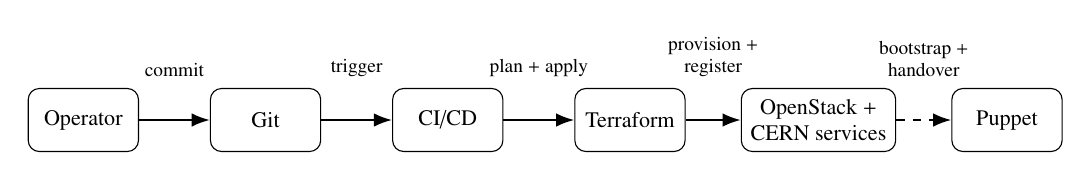
\begin{tikzpicture}[
  font=\footnotesize,
  block/.style={draw, rounded corners, align=center, minimum height=0.8cm, minimum width=1.4cm},
  arr/.style={-Latex, thick},
  lbl/.style={above=12pt, font=\scriptsize, align=center}
]

\node[block] (op) {Operator};
\node[block, right=0.9cm of op] (git) {Git};
\node[block, right=0.9cm of git] (ci) {CI/CD};
\node[block, right=0.9cm of ci] (tf) {Terraform};
\node[block, right=0.7cm of tf] (infra) {OpenStack +\\CERN services};
\node[block, right=0.7cm of infra] (puppet) {Puppet};

\draw[arr] (op) -- node[lbl]{commit} (git);
\draw[arr] (git) -- node[lbl]{trigger} (ci);
\draw[arr] (ci) -- node[lbl]{plan + apply} (tf);
\draw[arr] (tf) -- node[lbl]{provision +\\register} (infra);
\draw[arr, dashed] (infra) -- node[lbl]{bootstrap +\\handover} (puppet);

\end{tikzpicture}
}
  \caption{Provisioning workflow: infrastructure intent flows from Git through CI/CD and Terraform to infrastructure services. After bootstrap, Puppet assumes runtime configuration.}
  \label{fig:provisioning-seq}
\end{figure}

The point of the design is that provisioning and CM inputs come from one declarative definition, which is what removes the manual coordination at the provisioning/CM boundary. Updates go through the same \texttt{plan/apply} cycle.

\section{Implementation}\label{implementation}

The implementation keeps the interface that end users see as small as possible, and hides the provider-specific logic and the CERN-specific integrations inside reusable modules. Listing~\ref{lst:hostgroup} is the full input needed to deploy a host that comes up configured and registered. Provider configuration, bootstrap logic, and the integration with the supporting services all live inside the module.

\begin{listing}[ht]
    \begin{minted}[fontsize=\small]{HCL}
        module "my_hostgroup" {
          source  = "gitlab.cern.ch/terraform/terraform-cern-puppet-hostgroup/openstack"
          version = "1.0.0"

          foreman_hostgroup = "playground"

          instance_name_prefix = "service-x"

          landb_mainuser    = "username-or-group"
          landb_responsible = "username-or-group"
        }
    \end{minted}
    \caption{Minimal end-user instantiation of the module.}
    \label{lst:hostgroup}
\end{listing}

\subsection{Module Structure}
The provisioning layer is organised around a root module that composes the submodules from the declared inputs. The central abstraction is a \textit{node}, handled by an instances submodule that treats compute attributes, networking, identity material, classification metadata, and lifecycle registration as one logical unit. Persistent storage is deliberately kept out of that unit, in a separate volumes submodule, so that it can be managed on its own lifecycle.

\subsection{Custom Providers}
Where no provider existed, we wrote one. These custom Terraform/OpenTofu providers wrap the in-house services and expose their APIs as declarative resources, so service registrations and metadata updates go through the same plan/apply workflow as everything else.

\subsection{CI/CD Integration}
Infrastructure changes run through standardised CI/CD pipelines and nowhere else, which is what makes validation consistent and execution auditable. The pipeline logic is packaged as a reusable catalog component that a project pulls in with a single \texttt{include}. Every merge request triggers validation, linting, and a plan, and the plan is attached to the request as a human-readable artifact for review. Apply only runs once validation has passed and the required approvals are in, so there is no ad-hoc path to production.

\section{Evaluation and Results}\label{evaluation}

\subsection{Methodology}
We combined scenario-based testing with qualitative feedback from practitioners. A representative deployment scenario was run end-to-end to see how provisioning behaved, how it integrated with the existing services, and how it fitted the operational workflows. Alongside that, we collected feedback from people who deployed real services with the framework. The aim was to check correctness, consistency, and whether the thing is usable inside CERN's constraints, not to produce performance benchmarks.

\subsection{Results}
Applying the infrastructure definitions created, registered, and bootstrapped the target host with no manual intervention beyond writing the declaration. Re-applying the same declarations changed nothing, which confirms that the provisioning and registration layers are idempotent.

To test drift handling, we made changes by hand outside the framework. The next plan surfaced every deviation from the declared intent, giving an explicit and auditable list of what had diverged. Re-applying through the standard CI/CD workflow put it back. For controlled drift correction, the \texttt{plan/apply} cycle turned out to be enough on its own; continuous reconciliation was not needed.

Against the existing provisioning approach, the framework cut the number of manual coordination steps and closed off the ad-hoc execution paths. Reviewers also got something they did not have before: a plan artifact on the merge request showing exactly what was about to change, which meant less out-of-band checking before approving.

The operators we spoke to picked out the same thing, that they were leaning less on implicit coordination and on knowledge that was never written down, especially when infrastructure had to be recreated or migrated. Reproducing an environment at another site was reported as markedly easier, which is the BC/DR limitation identified in Section~\ref{infra}.

\section{Conclusion and Outlook}\label{conclusion}

We have presented an IaC framework that brings Terraform/OpenTofu into CERN's existing provisioning and CM ecosystem. It adds a declarative integration layer that holds infrastructure intent, provisioning, and service registration under one version-controlled roof. With custom providers for the in-house services and pipelines that gate every change, it cuts boundary drift, makes change traceable, and reduces how much undocumented operational knowledge a team needs to keep a service alive. That matters most in BC/DR and cross-environment replication.

Real deployments and operator feedback both point the same way: the framework makes operations more predictable, and it does so without disturbing the CM workflows people already rely on. Separating provisioning intent, execution, and ownership of runtime configuration works for infrastructure that is large, heterogeneous, and long-lived, which describes CERN's rather well.

There is more to do. Tying the framework to GitOps-style reconciliation controllers would allow continuous drift correction for selected resources, rather than waiting for an operator to re-apply. Adoption will be gradual: teams who know the existing workflows and have never used Terraform need time and support, and the migration path has to be incremental. Finally, making Policy-as-Code enforcement a design-time constraint rather than an optional check would put security and compliance guarantees on a firmer footing across every managed resource.


\begin{thebibliography}{}

\bibitem{bellinfra2012}
P. Andrade, T. Bell, J. van Eldik, G. McCance, B. Panzer-Steindel, M. Coelho dos Santos, S. Traylen, U. Schwickerath, J. Phys.: Conf. Ser. \textbf{396}, 042002 (2012)

\bibitem{loope2011managing}
J. Loope, \textit{Managing Infrastructure with Puppet: Configuration Management at Scale} (O'Reilly Media, 2011)

\bibitem{morris2025infrastructure}
K. Morris, \textit{Infrastructure as Code: Designing and Delivering Dynamic Systems for the Cloud Age} (O'Reilly Media, 2025)

\bibitem{savchenko2024preparing}
M. Savchenko, L. Atzori, N. Papakyprianou, M. Piszczek, A. Wiebalck, EPJ Web Conf. \textbf{295}, 07038 (2024)

\bibitem{dupuis2025}
M. Dupuis, EPJ Web Conf. \textbf{337}, 01148 (2025)

\bibitem{martelli2018}
E. Martelli, T. Cass, \textit{CERN Data Centre Network Architecture: proposed evolution and implementation plan}, Tech. Rep., CERN (2018), \url{https://cds.cern.ch/record/2628525}

\bibitem{alvarez2020batch}
L. Fernandez Alvarez, O. Datskova, B. Jones, G. McCance, EPJ Web Conf. \textbf{245}, 07048 (2020)

\end{thebibliography}


\end{document}
